% Options for packages loaded elsewhere
\PassOptionsToPackage{unicode}{hyperref}
\PassOptionsToPackage{hyphens}{url}
\PassOptionsToPackage{dvipsnames,svgnames,x11names}{xcolor}
%
\documentclass[
  letterpaper,
  DIV=11,
  numbers=noendperiod]{scrreprt}

\usepackage{amsmath,amssymb}
\usepackage{iftex}
\ifPDFTeX
  \usepackage[T1]{fontenc}
  \usepackage[utf8]{inputenc}
  \usepackage{textcomp} % provide euro and other symbols
\else % if luatex or xetex
  \usepackage{unicode-math}
  \defaultfontfeatures{Scale=MatchLowercase}
  \defaultfontfeatures[\rmfamily]{Ligatures=TeX,Scale=1}
\fi
\usepackage{lmodern}
\ifPDFTeX\else  
    % xetex/luatex font selection
\fi
% Use upquote if available, for straight quotes in verbatim environments
\IfFileExists{upquote.sty}{\usepackage{upquote}}{}
\IfFileExists{microtype.sty}{% use microtype if available
  \usepackage[]{microtype}
  \UseMicrotypeSet[protrusion]{basicmath} % disable protrusion for tt fonts
}{}
\makeatletter
\@ifundefined{KOMAClassName}{% if non-KOMA class
  \IfFileExists{parskip.sty}{%
    \usepackage{parskip}
  }{% else
    \setlength{\parindent}{0pt}
    \setlength{\parskip}{6pt plus 2pt minus 1pt}}
}{% if KOMA class
  \KOMAoptions{parskip=half}}
\makeatother
\usepackage{xcolor}
\setlength{\emergencystretch}{3em} % prevent overfull lines
\setcounter{secnumdepth}{5}
% Make \paragraph and \subparagraph free-standing
\makeatletter
\ifx\paragraph\undefined\else
  \let\oldparagraph\paragraph
  \renewcommand{\paragraph}{
    \@ifstar
      \xxxParagraphStar
      \xxxParagraphNoStar
  }
  \newcommand{\xxxParagraphStar}[1]{\oldparagraph*{#1}\mbox{}}
  \newcommand{\xxxParagraphNoStar}[1]{\oldparagraph{#1}\mbox{}}
\fi
\ifx\subparagraph\undefined\else
  \let\oldsubparagraph\subparagraph
  \renewcommand{\subparagraph}{
    \@ifstar
      \xxxSubParagraphStar
      \xxxSubParagraphNoStar
  }
  \newcommand{\xxxSubParagraphStar}[1]{\oldsubparagraph*{#1}\mbox{}}
  \newcommand{\xxxSubParagraphNoStar}[1]{\oldsubparagraph{#1}\mbox{}}
\fi
\makeatother

\usepackage{color}
\usepackage{fancyvrb}
\newcommand{\VerbBar}{|}
\newcommand{\VERB}{\Verb[commandchars=\\\{\}]}
\DefineVerbatimEnvironment{Highlighting}{Verbatim}{commandchars=\\\{\}}
% Add ',fontsize=\small' for more characters per line
\usepackage{framed}
\definecolor{shadecolor}{RGB}{241,243,245}
\newenvironment{Shaded}{\begin{snugshade}}{\end{snugshade}}
\newcommand{\AlertTok}[1]{\textcolor[rgb]{0.68,0.00,0.00}{#1}}
\newcommand{\AnnotationTok}[1]{\textcolor[rgb]{0.37,0.37,0.37}{#1}}
\newcommand{\AttributeTok}[1]{\textcolor[rgb]{0.40,0.45,0.13}{#1}}
\newcommand{\BaseNTok}[1]{\textcolor[rgb]{0.68,0.00,0.00}{#1}}
\newcommand{\BuiltInTok}[1]{\textcolor[rgb]{0.00,0.23,0.31}{#1}}
\newcommand{\CharTok}[1]{\textcolor[rgb]{0.13,0.47,0.30}{#1}}
\newcommand{\CommentTok}[1]{\textcolor[rgb]{0.37,0.37,0.37}{#1}}
\newcommand{\CommentVarTok}[1]{\textcolor[rgb]{0.37,0.37,0.37}{\textit{#1}}}
\newcommand{\ConstantTok}[1]{\textcolor[rgb]{0.56,0.35,0.01}{#1}}
\newcommand{\ControlFlowTok}[1]{\textcolor[rgb]{0.00,0.23,0.31}{\textbf{#1}}}
\newcommand{\DataTypeTok}[1]{\textcolor[rgb]{0.68,0.00,0.00}{#1}}
\newcommand{\DecValTok}[1]{\textcolor[rgb]{0.68,0.00,0.00}{#1}}
\newcommand{\DocumentationTok}[1]{\textcolor[rgb]{0.37,0.37,0.37}{\textit{#1}}}
\newcommand{\ErrorTok}[1]{\textcolor[rgb]{0.68,0.00,0.00}{#1}}
\newcommand{\ExtensionTok}[1]{\textcolor[rgb]{0.00,0.23,0.31}{#1}}
\newcommand{\FloatTok}[1]{\textcolor[rgb]{0.68,0.00,0.00}{#1}}
\newcommand{\FunctionTok}[1]{\textcolor[rgb]{0.28,0.35,0.67}{#1}}
\newcommand{\ImportTok}[1]{\textcolor[rgb]{0.00,0.46,0.62}{#1}}
\newcommand{\InformationTok}[1]{\textcolor[rgb]{0.37,0.37,0.37}{#1}}
\newcommand{\KeywordTok}[1]{\textcolor[rgb]{0.00,0.23,0.31}{\textbf{#1}}}
\newcommand{\NormalTok}[1]{\textcolor[rgb]{0.00,0.23,0.31}{#1}}
\newcommand{\OperatorTok}[1]{\textcolor[rgb]{0.37,0.37,0.37}{#1}}
\newcommand{\OtherTok}[1]{\textcolor[rgb]{0.00,0.23,0.31}{#1}}
\newcommand{\PreprocessorTok}[1]{\textcolor[rgb]{0.68,0.00,0.00}{#1}}
\newcommand{\RegionMarkerTok}[1]{\textcolor[rgb]{0.00,0.23,0.31}{#1}}
\newcommand{\SpecialCharTok}[1]{\textcolor[rgb]{0.37,0.37,0.37}{#1}}
\newcommand{\SpecialStringTok}[1]{\textcolor[rgb]{0.13,0.47,0.30}{#1}}
\newcommand{\StringTok}[1]{\textcolor[rgb]{0.13,0.47,0.30}{#1}}
\newcommand{\VariableTok}[1]{\textcolor[rgb]{0.07,0.07,0.07}{#1}}
\newcommand{\VerbatimStringTok}[1]{\textcolor[rgb]{0.13,0.47,0.30}{#1}}
\newcommand{\WarningTok}[1]{\textcolor[rgb]{0.37,0.37,0.37}{\textit{#1}}}

\providecommand{\tightlist}{%
  \setlength{\itemsep}{0pt}\setlength{\parskip}{0pt}}\usepackage{longtable,booktabs,array}
\usepackage{calc} % for calculating minipage widths
% Correct order of tables after \paragraph or \subparagraph
\usepackage{etoolbox}
\makeatletter
\patchcmd\longtable{\par}{\if@noskipsec\mbox{}\fi\par}{}{}
\makeatother
% Allow footnotes in longtable head/foot
\IfFileExists{footnotehyper.sty}{\usepackage{footnotehyper}}{\usepackage{footnote}}
\makesavenoteenv{longtable}
\usepackage{graphicx}
\makeatletter
\newsavebox\pandoc@box
\newcommand*\pandocbounded[1]{% scales image to fit in text height/width
  \sbox\pandoc@box{#1}%
  \Gscale@div\@tempa{\textheight}{\dimexpr\ht\pandoc@box+\dp\pandoc@box\relax}%
  \Gscale@div\@tempb{\linewidth}{\wd\pandoc@box}%
  \ifdim\@tempb\p@<\@tempa\p@\let\@tempa\@tempb\fi% select the smaller of both
  \ifdim\@tempa\p@<\p@\scalebox{\@tempa}{\usebox\pandoc@box}%
  \else\usebox{\pandoc@box}%
  \fi%
}
% Set default figure placement to htbp
\def\fps@figure{htbp}
\makeatother
% definitions for citeproc citations
\NewDocumentCommand\citeproctext{}{}
\NewDocumentCommand\citeproc{mm}{%
  \begingroup\def\citeproctext{#2}\cite{#1}\endgroup}
\makeatletter
 % allow citations to break across lines
 \let\@cite@ofmt\@firstofone
 % avoid brackets around text for \cite:
 \def\@biblabel#1{}
 \def\@cite#1#2{{#1\if@tempswa , #2\fi}}
\makeatother
\newlength{\cslhangindent}
\setlength{\cslhangindent}{1.5em}
\newlength{\csllabelwidth}
\setlength{\csllabelwidth}{3em}
\newenvironment{CSLReferences}[2] % #1 hanging-indent, #2 entry-spacing
 {\begin{list}{}{%
  \setlength{\itemindent}{0pt}
  \setlength{\leftmargin}{0pt}
  \setlength{\parsep}{0pt}
  % turn on hanging indent if param 1 is 1
  \ifodd #1
   \setlength{\leftmargin}{\cslhangindent}
   \setlength{\itemindent}{-1\cslhangindent}
  \fi
  % set entry spacing
  \setlength{\itemsep}{#2\baselineskip}}}
 {\end{list}}
\usepackage{calc}
\newcommand{\CSLBlock}[1]{\hfill\break\parbox[t]{\linewidth}{\strut\ignorespaces#1\strut}}
\newcommand{\CSLLeftMargin}[1]{\parbox[t]{\csllabelwidth}{\strut#1\strut}}
\newcommand{\CSLRightInline}[1]{\parbox[t]{\linewidth - \csllabelwidth}{\strut#1\strut}}
\newcommand{\CSLIndent}[1]{\hspace{\cslhangindent}#1}

\KOMAoption{captions}{tableheading}
\makeatletter
\@ifpackageloaded{bookmark}{}{\usepackage{bookmark}}
\makeatother
\makeatletter
\@ifpackageloaded{caption}{}{\usepackage{caption}}
\AtBeginDocument{%
\ifdefined\contentsname
  \renewcommand*\contentsname{Índice}
\else
  \newcommand\contentsname{Índice}
\fi
\ifdefined\listfigurename
  \renewcommand*\listfigurename{Lista de Figuras}
\else
  \newcommand\listfigurename{Lista de Figuras}
\fi
\ifdefined\listtablename
  \renewcommand*\listtablename{Lista de Tabelas}
\else
  \newcommand\listtablename{Lista de Tabelas}
\fi
\ifdefined\figurename
  \renewcommand*\figurename{Figura}
\else
  \newcommand\figurename{Figura}
\fi
\ifdefined\tablename
  \renewcommand*\tablename{Tabela}
\else
  \newcommand\tablename{Tabela}
\fi
}
\@ifpackageloaded{float}{}{\usepackage{float}}
\floatstyle{ruled}
\@ifundefined{c@chapter}{\newfloat{codelisting}{h}{lop}}{\newfloat{codelisting}{h}{lop}[chapter]}
\floatname{codelisting}{Listagem}
\newcommand*\listoflistings{\listof{codelisting}{Lista de Listagens}}
\makeatother
\makeatletter
\makeatother
\makeatletter
\@ifpackageloaded{caption}{}{\usepackage{caption}}
\@ifpackageloaded{subcaption}{}{\usepackage{subcaption}}
\makeatother

\ifLuaTeX
\usepackage[bidi=basic]{babel}
\else
\usepackage[bidi=default]{babel}
\fi
\babelprovide[main,import]{brazilian}
% get rid of language-specific shorthands (see #6817):
\let\LanguageShortHands\languageshorthands
\def\languageshorthands#1{}
\usepackage{bookmark}

\IfFileExists{xurl.sty}{\usepackage{xurl}}{} % add URL line breaks if available
\urlstyle{same} % disable monospaced font for URLs
\hypersetup{
  pdftitle={Introdução à Geoinformática},
  pdfauthor={Édipo H. Cremon},
  pdflang={pt-BR},
  colorlinks=true,
  linkcolor={blue},
  filecolor={Maroon},
  citecolor={Blue},
  urlcolor={Blue},
  pdfcreator={LaTeX via pandoc}}


\title{Introdução à Geoinformática}
\author{Édipo H. Cremon}
\date{2026-03-10}

\begin{document}
\maketitle

\renewcommand*\contentsname{Índice}
{
\hypersetup{linkcolor=}
\setcounter{tocdepth}{2}
\tableofcontents
}

\bookmarksetup{startatroot}

\chapter{Apresentação}\label{apresentauxe7uxe3o}

Este material didático foi elaborado com o objetivo de oferecer uma base
conceitual e metodológica para o estudo da Geoinformática, área dedicada
ao desenvolvimento e à aplicação de métodos computacionais voltados à
análise de fenômenos que possuem localização na superfície terrestre e
apresentam variação no tempo e no espaço. O avanço das tecnologias de
aquisição, armazenamento e processamento de dados geográficos tem
ampliado significativamente as possibilidades de investigação científica
e de suporte à tomada de decisão em diferentes domínios de aplicação.

Nas últimas décadas, a crescente disponibilidade de dados geoespaciais
provenientes de sensores orbitais, redes de monitoramento ambiental,
dispositivos móveis e iniciativas de produção colaborativa de informação
geográfica ampliou a complexidade dos problemas associados à gestão e
análise de dados espaciais. Nesse contexto, a Geoinformática integra
conceitos provenientes da ciência da computação, da geografia, da
estatística e da ciência de dados para desenvolver métodos capazes de
representar, armazenar, processar e analisar grandes volumes de dados
geográficos e espaço-temporais.

Este material organiza os principais conceitos necessários para
compreender o funcionamento dos sistemas de informação geográfica e das
tecnologias associadas ao processamento de dados espaciais.

O material foi desenvolvido (e está em desenvolvimento) para apoiar
atividades de ensino em disciplinas de Geoinformática e áreas
correlatas, combinando fundamentos teóricos com exemplos aplicados e
referências à literatura científica. Espera-se que, ao final do estudo,
o leitor seja capaz de compreender os principais conceitos associados à
análise de dados geoespaciais e utilizá-los no desenvolvimento de
projetos de pesquisa ou aplicações voltadas à resolução de problemas
reais.

\bookmarksetup{startatroot}

\chapter{Conceitos: quem é quem no mundo
``geo''?}\label{conceitos-quem-uxe9-quem-no-mundo-geo}

A compreensão contemporânea do espaço geográfico e sua representação
digital exigem uma análise de um ecossistema terminológico que, embora
compartilhe a raiz comum do estudo da Terra, apresenta distinções
ontológicas, epistemológicas e instrumentais significativas. O advento
da era digital transformou a cartografia analítica em um campo vasto e
interdisciplinar, onde a geoinformática, a geomática, o
geoprocessamento, as geotecnologias, a ciência de dados espaciais e a
GIScience (Ciência da Informação Geográfica) se entrelaçam em uma rede
complexa de significados.

A coexistência de múltiplas terminologias gera ambiguidades conceituais
que afetam tanto a produção acadêmica quanto a aplicação técnica em
órgãos governamentais e empresas. Pesquisas indicam que as preferências
terminológicas variam conforme a localização geográfica e a tradição
acadêmica; a geomática possui forte influência francesa e canadense,
enquanto a geoinformática predomina na literatura europeia central e
alemã. No Brasil, os conceitos de geoprocessamento e geotecnologias
possuem definições que muitas vezes se sobrepõem erroneamente em editais
e publicações técnicas, dificultando a distinção entre o processamento
analítico e o conjunto instrumental de suporte.

Este texto explora cada um desses conceitos, detalhando suas origens
etimológicas, suas evoluções históricas, as nuances que os distinguem e
a estrutura hierárquica que define sua aplicação no monitoramento e na
gestão do mundo físico.

\section{Geoinformática}\label{geoinformuxe1tica}

A identidade conceitual da geoinformática está enraizada em sua
etimologia, o termo ``Geoinformática'' é um neologismo composto pelo
prefixo grego geo- (\$\textbackslash gamma
\textbackslash tilde\{\textbackslash eta\}\$), que significa ``Terra'',
e pelo substantivo ``Informática''. Este último termo é, por sua vez,
uma aglutinação de ``Informação'' e ``Automática'', sugerindo o
processamento automatizado da informação. Assim, a geoinformática é, em
sua essência, o tratamento automático de informações relativas à Terra.
O termo foi introduzido por Samuelson em 1988, na Suécia (Krawczyk
(2022)).

Na literatura formal, a geoinformática é definida como a ciência e
tecnologia que lida com a estrutura e o caráter da informação espacial,
sua captura, classificação, armazenamento, processamento e disseminação
(Olędzki; Kwiatkowska (2004)). Mais recentemente, a geoinformática foi
redefinida como uma ciência técnica dentro da Ciência da Computação,
focada na programação de aplicações, estruturas de dados espaciais e
análise de objetos e fenômenos espaço-temporais, incluindo o
desenvolvimento de serviços web para modelagem espacial (Krawczyk
(2022)).

Esta definição contemporânea reflete a evolução do conceito desde sua
origem, posicionando a geoinformática como uma ponte entre as
geociências e a ciência da computação. Nessa perspectiva, a
geoinformática não se limita ao uso de ferramentas prontas, mas se
dedica à criação de novas estruturas de dados, algoritmos e arquiteturas
computacionais para lidar com a complexidade dos fenômenos
espaço-temporais.

A visão de longo prazo para a área é a construção de sistemas de dados
altamente interconectados, povoados com dados de qualidade e livremente
disponíveis, acompanhados de um conjunto robusto de softwares para
análise, visualização e modelagem (Brady; Sinha; Gundersen (2007)).

Historicamente, o termo geoinformática ganhou força na Europa,
especialmente na Alemanha.No Brasil, a introdução desse conceito ocorreu
impulsionada pelo Instituto Nacional de Pesquisas Espaciais (INPE), que
inclusive organiza periodicamente, desde 1999, o
\href{http://www.geoinfo.info/}{Simpósio Brasileiro de Geoinformática
(GeoInfo)}.

O protagonismo do INPE na consolidação da geoinformática no Brasil vai
além da organização do \href{http://www.geoinfo.info/}{GeoInfo}. O
Instituto tem contribuído ativamente para o desenvolvimento tecnológico
da área, com iniciativas como o SPRING, um software de Sistema de
Informação Geográfica, e o e desenvolvimento da
\href{http://www.dpi.inpe.br/terralib}{TerraLib,} biblioteca de código
aberto para suportar aplicações em Geoinformática que resultou no
software TerraView. Mais recentemente, projetos como o Brazil Data Cube
exemplificam a vanguarda da pesquisa brasileira em geoinformática,
aplicando tecnologias de big data, aprendizado de máquina e análise de
séries temporais de imagens de satélite para produzir informação oficial
sobre desmatamento, queimadas e uso e cobertura da terra para o governo
brasileiro. Atualmente, a Divisão de Observação da Terra e
Geoinformática do INPE segue coordenando projetos que posicionam o
Brasil na fronteira do conhecimento da área.

\section{Geomática}\label{geomuxe1tica}

O conceito de Geomática representa um dos primeiros e mais robustos
esforços de unificação terminológica no campo geoespacial. Sua origem
remonta ao final da década de 1960, quando o franco-canadense Bernard
Dubuisson, cientista com formação em agrimensura e fotogrametria, propôs
o termo ``\emph{géomatique}'' para refletir as profundas transformações
que as profissões de agrimensor e fotogrametrista começavam a
experimentar diante do avanço da automação e da computação. Dubuisson
criou o neologismo ao propor a junção do prefixo ``geo'' (referência à
Terra) com o sufixo ``matique'' , extraído da palavra
``\emph{informatique}'' (informática em francês), com o objetivo de
designar de forma integrada as então distintas disciplinas de aquisição
e processamento de dados da Terra sob um novo paradigma tecnológico. A
palavra ``\emph{géomatique}'' foi posteriormente anglicizada para
``\emph{Geomatics}'' e oficialmente adotada no Canadá, especialmente na
década de 1980 e 1990, como parte de uma reforma educacional e
profissional para modernizar e unificar as áreas de agrimensura,
cartografia e topografia sob um novo paradigma tecnológico (Krawczyk
(2022)).

A geomática representa um campo de atividades científicas, tecnológicas
e artísticas que, por meio de uma abordagem sistêmica e integrada, se
dedica à aquisição, medição, análise, gestão, armazenamento e
disseminação de dados e informações geoespaciais. Tem raízes fortes na
engenharia, particularmente na agrimensura, cartografia e geodesia.
Krawczyk (2022) situa sua origem como uma tentativa de modernizar e
ampliar o escopo da geodésia, focando no processo completo de
gerenciamento da informação espacial, desde a coleta em campo até a
entrega ao usuário.

A definição formal adotada pela série de normas ISO/TC 211 estabelece a
Geomática como a disciplina preocupada com a coleta, distribuição,
armazenamento, análise, processamento e apresentação de dados
geográficos ou informação geográfica (Brodeur (2001)).

A Geomática é frequentemente descrita como um termo guarda-chuva que
inclui ferramentas e técnicas variadas, desde a agrimensura terrestre
clássica até o sensoriamento remoto aéreo e orbital, sistemas de
posicionamento global (GNSS) e cartografia náutica (Krawczyk (2022)). De
acordo com a redefinição proposta por Krawczyk (2022), a Geomática deve
ser situada no âmbito das Ciências da Terra em conexão com as ciências
técnicas, tendo como objetivo principal o desenvolvimento de métodos e
técnicas para a aquisição e gestão de dados espaciais relacionados à
superfície terrestre, visando a modelagem e visualização de fenômenos
espaço-temporais.

Em termos de aceitação global, a Geomática é o termo preferencial no
Canadá, na Austrália, na Nova Zelândia e na França.Nesses países, o
termo é amplamente utilizado em nomes de departamentos universitários,
conselhos profissionais e órgãos governamentais.No entanto, nos Estados
Unidos, o termo encontrou resistência, sendo muitas vezes preterido por
GIScience.

Essa distribuição geográfica de uso reflete diferentes tradições
acadêmicas e percursos históricos. Enquanto no Canadá e na França a
adoção do termo esteve ligada a políticas explícitas de modernização
profissional e educacional, nos Estados Unidos a preferência por
GIScience (Ciência da Informação Geográfica) evidencia uma tradição de
maior ênfase nos fundamentos teóricos e cognitivos da informação
geoespacial, em detrimento da abordagem mais voltada à engenharia de
agrimensura característica da geomática. Essa tensão terminológica,
longe de ser um problema, demonstra a riqueza e a complexidade do campo,
que comporta múltiplas perspectivas igualmente legítimas para o estudo
do espaço geográfico.

\section{GIScience / Ciência da
Geoinformação}\label{giscience-ciuxeancia-da-geoinformauxe7uxe3o}

A expressão GIScience (\emph{Geographic Information Science}) pode ser
interpretada literalmente como ``ciência da informação geográfica'', ou
seja, o estudo científico da informação associada à localização e aos
processos espaciais. Na América Latina, e em particular no Brasil, a
literatura acadêmica frequentemente utiliza a expressão ``Ciência da
Geoinformação'', adotada por autores como Câmara; Monteiro (2001), como
tradução conceitual próxima à GIScience.

A GIScience constitui um campo científico dedicado ao estudo sistemático
da informação geográfica, de suas propriedades, métodos de representação
e processos de análise (Longley et al. (2015)). Essa interpretação
converge com a definição apresentada por Câmara; Monteiro (2001),
segundo a qual um dos problemas fundamentais da ciência da geoinformação
consiste no estudo e na construção de modelos computacionais destinados
à representação do espaço geográfico.

O termo GIScience foi introduzido no início da década de 1990 pelo
estadunidense Michael F. Goodchild para designar o conjunto de questões
científicas fundamentais relacionadas às tecnologias de informação
geográfica, particularmente aos Sistemas de Informação Geográfica (GIS)
(Goodchild (1992)). A formulação de Goodchild representou a transição de
uma abordagem predominantemente tecnológica, centrada em sistemas
computacionais de manipulação espacial (software), para uma abordagem
científica (teoria) voltada à investigação dos fenômenos relacionados à
informação geográfica (Goodchild (1992)). Enquanto o SIG foca no ``como
fazer'', a GIScience foca no ``o que sabemos'' e em como a informação
geográfica representa fenômenos do mundo real e a percepção humana.

A GIScience ou Ciência da Geoinformação não é somente o estudo de mapas
digitais. É uma área independente que examina a natureza fundamental do
espaço geográfico e do tempo, a cognição humana e os métodos
computacionais necessários para capturar essa realidade complexa
(Câmara; Monteiro (2001)). Ela se diferencia do SIG por sua natureza
reflexiva e investigativa, buscando leis e princípios universais que
governem a informação geoespacial (Longley et al. (2015)).

Em um panorama geral, o termo GIScience é o mais consolidado nos Estados
Unidos. Sua adoção foi impulsionada pela necessidade dos geógrafos
estadunidenses de afirmar a legitimidade científica de suas pesquisas
frente à computação (Goodchild (1992)). O termo é amplamente utilizado
em departamentos de geografia e pela
\href{https://www.ucgis.org/}{UCGIS} (\emph{University Consortium for
Geographic Information Science}, National Research Council (2006)).

\section{Geoprocessamento}\label{geoprocessamento}

O termo geoprocessamento deriva da combinação de dois componentes. O
prefixo ``geo'' provém do grego, que significa Terra. Já o termo
``processamento'' tem origem no latim \emph{processus}, que significa
avançar ou realizar operações em sequência. Assim, o significado literal
de geoprocessing é ``processamento de dados relacionados à Terra''.

Na América do Norte e na maioria dos países europeus, o termo
geoprocessamento é geralmente empregado em um sentido operacional mais
específico. Ele se refere principalmente a ferramentas computacionais
realizadas em ambientes de software de SIG. ``\emph{Geoprocessing}'' é
utilizado como um termo técnico por profissionais da área,
particularmente por aqueles inseridos no ecossistema Esri, para
descrever automação e fluxos de trabalho de modelagem geoespacial. Na
literatura acadêmica, discussões conceituais mais amplas tendem a
preferir termos como GIScience, geoinformática ou geomática.

No Brasil e em outros países da América Latina, o termo
``geoprocessamento'' passou a ser amplamente adotado a partir da década
de 1990, em grande parte influenciado pela tradição acadêmica
estabelecida pelo INPE. Os livros do INPE organizados por Câmara, Davis
e Monteiro e o desenvolvimento do software
\href{http://www.dpi.inpe.br/spring/}{SPRING}, acrônimo para ``Sistema
de Processamento de Informações Georeferenciadas'', contribuiram para
institucionalizar o geoprocessamento como uma disciplina científica
própria e desempenharam um papel central na difusão do termo na
literatura em língua portuguesa e nos currículos acadêmicos. Nesse
contexto, geoprocessamento é comumente utilizado como um conceito
abrangente, que se refere a tecnologias e métodos voltados ao
processamento de dados geoespaciais.

Na obra seminal
``\href{http://www.dpi.inpe.br/gilberto/livro/introd/index.html}{Introdução
à ciência da geoinformação}'', produzida pelo INPE no Brasil, Câmara;
Davis; Monteiro (2001) apresentam uma definição que eleva o conceito
para além de meras operações de software. Os autores definem
geoprocessamento como uma tecnologia interdisciplinar que possibilita a
convergência de diversas disciplinas científicas para o estudo de
fenômenos urbanos e ambientais. Um entendimento fundamental da escola do
INPE é que ``o espaço funciona como uma linguagem comum'' para
diferentes campos do conhecimento; contudo, essa interdisciplinaridade é
tecnicamente viabilizada por meio da redução de conceitos específicos de
cada disciplina em algoritmos e estruturas de dados adequados ao
tratamento computacional.

Segundo esses autores, geoprocessamento abrange a infraestrutura
tecnológica e metodológica necessária para capturar, armazenar,
processar, analisar e apresentar informações geográficas por meio de
sistemas computacionais. Nesse quadro conceitual, os SIGs constituem a
principal plataforma tecnológica para a implementação de operações de
geoprocessamento, permitindo a integração de dados espaciais
provenientes de múltiplas fontes e a automação de procedimentos
analíticos (Câmara; Davis; Monteiro (2001)). Diferente do SIG (o
sistema), o geoprocessamento é visto no Brasil como o campo
técnico-científico que abrange a integração de diversas tecnologias,
como o próprio SIG, o Sensoriamento Remoto, o GNSS e a Cartografia
Digital.

\section{Geotecnologia}\label{geotecnologia}

O termo geotecnologia origina-se da combinação de expressões
relacionadas às tecnologias geoespaciais e refere-se principalmente ao
mercado tecnológico associado à aquisição e ao processamento de dados
geoespaciais, e não a um campo de pesquisa científica. Essa
interpretação destaca que geotecnologia descreve o ecossistema de
soluções tecnológicas utilizado em atividades geoespaciais, incluindo
equipamentos e sistemas projetados para aquisição e análise de dados.

O surgimento do termo está estreitamente associado aos desenvolvimentos
da indústria geoespacial nos Estados Unidos, onde passou a ser
amplamente utilizado no mercado de trabalho e no setor tecnológico para
designar profissões e indústrias vinculadas ao processamento de dados
geoespaciais. Nesse contexto, o conceito refere-se ao domínio econômico
e tecnológico que abrange empresas que fabricam instrumentos e
desenvolvem softwares e serviços para análise espacial e navegação
(Gewin, 2004). Por exemplo, fabricantes de receptores GNSS, instrumentos
de levantamento e sensores de sensoriamento remoto são frequentemente
considerados parte do setor de geotecnologias (Gewin (2004)).

Devido a esse significado tecnológico e orientado ao mercado, o termo
pode, por vezes, ser confundido com geotecnia, uma área da engenharia
civil voltada à mecânica dos solos e à engenharia de fundações (e.g.
Roberts (1977)). Essa similaridade terminológica pode levar a
interpretações equivocadas, especialmente fora do campo das ciência da
geoinformação. Como resultado, alguns autores argumentam que a expressão
geotecnologia não é adequada para designar o campo científico dedicado
aos estudos da informação geoespacial, uma vez que carece de uma conexão
explícita com a teoria científica e pode se sobrepor à terminologia
utilizada em outros domínios da engenharia (Krawczyk (2022)).

Em países de língua inglesa, particularmente nos Estados Unidos, o
conceito está fortemente associado à indústria geoespacial e ao mercado
de trabalho, sobretudo em discussões sobre carreiras e inovação
tecnológica nos campos da geoinformação (Gewin (2004)). No Brasil e em
outros países da América Latina, a forma plural ``geotecnologias'' é
amplamente utilizada em contextos acadêmicos e aplicados para se
referir, de forma coletiva, a tecnologias como SIG, sensoriamento remoto
e navegação por satélite empregadas na análise geográfica. Apesar dessas
variações regionais, o conceito refere-se de maneira consistente à
infraestrutura tecnológica que sustenta a aquisição, o processamento e a
aplicação de dados geoespaciais.

\textbf{Dado vs.~Informação}

Os termos dado e informação são frequentemente utilizados como
sinônimos, porém representam conceitos distintos.

Dados correspondem a registros brutos, símbolos ou valores que descrevem
algum fenômeno, mas que ainda não foram interpretados. Eles podem estar
organizados em números, textos, códigos ou imagens, sem que
necessariamente possuam significado imediato para quem os observa.

Informação, por sua vez, resulta do processo de interpretação dos dados.
Quando um conjunto de dados é compreendido dentro de um contexto e passa
a transmitir significado, ele se transforma em informação.

Um exemplo simples ajuda a ilustrar essa diferença. Imagine um livro
escrito em russo para uma pessoa que não conhece o alfabeto cirílico.
Para essa pessoa, o texto consiste apenas em uma sequência de caracteres
sem significado, ou seja, um conjunto de dados. No entanto, para alguém
que domina o idioma, os mesmos caracteres podem ser decodificados,
interpretados e compreendidos. Nesse caso, o conteúdo do livro passa a
representar informação.

\section{Ciência de Dados
Geoespaciais}\label{ciuxeancia-de-dados-geoespaciais}

A Ciência de Dados Geospaciais, ou Ciência de Dados Geográficos, ou
ainda, Ciência de Dados Espaciais (\emph{Spatial Data Science}) está
alinhada a um conceito mais recente na hierarquia geoespacial, surgindo
da intersecção entre a ciência de dados moderna e a GIScience
tradicional (Scheider et al. (2020)). Luc Anselin descreve esse
movimento como uma ``morfose'' da GIScience para a ciência de dados
espaciais, onde a geografia quantitativa se dissolve em uma das muitas
ciências de dados que tratam de informações geográficas (Scheider et al.
(2020)).

Etimologicamente, o termo combina ``Ciência de Dados'' (estudo dos dados
e sua extração de conhecimento) com o qualificativo ``Geoespacial''. A
escolha do termo ``\emph{data}'' em vez de ``\emph{information}'' no
nome do campo é deliberada. Hu (2020) atribui essa opção à recente
popularização do termo ``\emph{data science}'' e à crescente importância
dos dados em si, seu volume, variedade e papel como facilitadores de
novos métodos, como aprendizado de máquina. Esse movimento marca uma
mudança sutil em relação à década de 1990, quando Michael Goodchild
cunhou o termo ``\emph{Geographic Information Science}'', em parte para
alinhar-se ao acrônimo já estabelecido ``GIS'', embora seu trabalho
fundamental estivesse voltado aos dados (Hu (2020)).

Do ponto de vista conceitual, a Ciência de Dados (Geo)Espaciais pode ser
entendida como um subcampo da ciência de dados que se dedica às
características particulares dos dados geoespaciais. Nesse contexto, a
dimensão espacial, expressa pela localização, pela distância e pelas
interações espaciais, constitui um elemento fundamental da análise. Como
destaca Anselin (2019), a ciência de dados espaciais trata
explicitamente do ``onde'' presente nos dados e emprega métodos, modelos
e infraestruturas computacionais capazes de armazenar, recuperar,
explorar, analisar, visualizar e extrair conhecimento a partir de dados
com referência espacial. Nessa perspectiva, a relação entre ciência de
dados espaciais e ciência de dados é análoga à relação entre estatística
espacial e estatística, bancos de dados geográficos e bancos de dados
convencionais, ou ainda geocomputação e computação em geral (Anselin
(2019)).

O diferencial da Ciência de Dados Geospaciais é a aplicação de métodos
de aprendizado de máquina (\emph{machine learning}), inteligência
artificial (IA) e estatística avançada a volumes massivos de dados
geográficos (Big Data). Diferente do SIG tradicional, que muitas vezes é
limitado por ferramentas de desktop, a Ciência de Dados Geospaciais
utiliza computação em nuvem e algoritmos orientados a dados para
descobrir padrões que não seriam visíveis por métodos puramente
cartográficos.

Há um debate contínuo sobre se a Ciência de Dados Geospaciais é uma
disciplina científica autônoma ou uma ``comunidade de prática''
(Scheider et al. (2020)). Para se tornar uma ciência de pleno direito
(uma meta-ciência), pesquisadores afirmam que ela precisa desenvolver
suas próprias teorias sobre métodos, indo além da simples aplicação de
modelos de IA a problemas espaciais (Scheider et al. (2020)).

O termo \emph{Spatial Data Science} ganhou destaque principalmente em
ambientes acadêmicos de língua inglesa, especialmente nos Estados Unidos
e no Reino Unido. Universidades como \emph{University College London},
\emph{University of Chicago} e \emph{University of Liverpool}
estabeleceram programas de pós-graduação e grupos de pesquisa dedicados
à ciência de dados geográficos ou ciência de dados espaciais. Em outras
regiões, incluindo América Latina e Ásia, a terminologia vem sendo
gradualmente incorporada à pesquisa, ao ensino e ao mercado de trabalho.

\textbf{Informação geográfica, geoespacial, espacial e geoinformação}

No contexto da ciência da geoinformação, diferentes termos são
utilizados para descrever dados e informações associados à localização.
Entre os mais comuns estão informação geográfica, informação geoespacial
e informação espacial. Embora muitas vezes empregados como sinônimos,
esses termos apresentam diferenças conceituais sutis.

A expressão informação geográfica refere-se a dados ou informações
associados à superfície terrestre e ao seu entorno imediato, abrangendo
fenômenos naturais e sociais que possuem localização no espaço
geográfico. Esse termo é tradicionalmente utilizado na literatura de
Sistemas de Informação Geográfica (SIG) e enfatiza o estudo de fenômenos
que ocorrem na Terra (Longley et al. (2015)).

A expressão informação geoespacial surgiu mais recentemente e costuma
ser utilizada para designar um subconjunto da informação espacial
aplicado especificamente à Terra, podendo estar em superfície,
subsuperfície ou na atmosfera. Em muitos contextos institucionais e
tecnológicos, especialmente no setor de geotecnologias, esse termo
tornou-se amplamente difundido (Longley et al. (2015)). Geoinformação é
sinônimo de informação geoespacial.

Já o termo informação espacial possui um significado mais amplo. Ele se
refere a qualquer informação associada a posições em um espaço,
independentemente de esse espaço ser terrestre. Assim, métodos
desenvolvidos para análise de informação geográfica podem ser aplicados
a outros domínios, como a superfície de outros planetas, o espaço
cósmico ou estruturas biológicas obtidas por imagens médicas (Longley et
al. (2015)).

\begin{center}
\pandocbounded{\includegraphics[keepaspectratio]{fig/conceitos_geo.png}}
\end{center}

Na prática, para a maioria das aplicações, os três termos podem ser
usados de forma intercambiável, desde que o contexto deixe claro o
domínio terrestre (quando for o caso). A escolha entre eles reflete
muitas vezes apenas uma tradição de área ou preferência editorial
(Longley et al. (2015)).

\section{Sistemas de Informação Geográfica
(SIG)}\label{sistemas-de-informauxe7uxe3o-geogruxe1fica-sig}

Os Sistemas de Informação Geográfica (SIG, ou GIS do acrônimo em inglês
\emph{Geographic Information Systems}) são definidos como conjuntos
computacionais de ferramentas destinadas à coleta, armazenamento,
recuperação, manipulação, análise e visualização de dados espaciais
representativos do mundo real (Burrough (1986); Aronoff (1989); Clarke;
Parks; Crane (2006)). Em uma abordagem orientada à gestão, o SIG pode
ser entendido como um sistema de suporte à decisão que integra dados
geoespaciais em um ambiente voltado à resolução de problemas, operando
sobre um banco de dados geográfico (Longley et al. (2015)).

Devido à ampla diversidade de aplicações, que inclui áreas como
agricultura, gestão florestal, cartografia, cadastro urbano e
gerenciamento de redes de infraestrutura, como água, energia e
telecomunicações, os SIGs podem ser utilizados de diferentes maneiras.
De acordo com Câmara; Queiroz (2001), em relação as funções genéricas de
um SIG, existem pelo menos três formas principais de utilização desses
sistemas:

\begin{itemize}
\item
  como ferramenta para produção cartográfica;
\item
  como suporte para análise espacial de fenômenos; e
\item
  como um banco de dados geográficos, com funções de armazenamento,
  organização e recuperação de informação geoespacial.
\end{itemize}

O desenvolvimento dos SIG está associado ao avanço da capacidade de
armazenamento de dados e ao aumento do poder de processamento dos
computadores de grande porte durante a segunda metade do século XX.
Nesse contexto, o geógrafo Roger Tomlinson é amplamente reconhecido como
o precursor dessa área, ao liderar o desenvolvimento do \emph{Canadian
Geographic Information System} (CGIS), criado para armazenar, analisar e
manipular dados produzidos pelo \emph{Canada Land Inventory} (Tomlinson
(1967)).
\href{https://gisandscience.wordpress.com/wp-content/uploads/2012/08/4-computermapping.pdf}{Em
relatório publicado em 1962}, Tomlinson já indicava a viabilidade do uso
de computadores para o armazenamento, compilação e avaliação de mapas e
dados estatísticos.

A etimologia do termo SIG remonta a esse contexto histórico. Ao longo
das décadas seguintes, o conceito evoluiu e a própria sigla passou por
diferentes interpretações. Alguns autores propuseram expansões
terminológicas que substituem \emph{Systems} por \emph{Science},
\emph{Studies} ou \emph{Society}, e \emph{Geographic} por
\emph{Geospatial}, buscando ampliar o alcance conceitual do termo e
destacar dimensões científicas ou sociais associadas ao uso dessas
tecnologias (Krawczyk (2022)).

O desenvolvimento institucional e tecnológico dos SIG consolidou-se ao
longo da década de 1970. Em 1975, pesquisadores do \emph{Laboratory for
Computer Graphics and Spatial Analysis}, da \emph{Harvard University},
implementaram um dos primeiros sistemas acadêmicos estruturados para
manipulação de dados espaciais. No final da década, a ampliação da
memória computacional e o avanço das capacidades gráficas dos
computadores favoreceram o surgimento dos primeiros softwares comerciais
de SIG (Waters (2017)). Em termos operacionais, um SIG pode ser
entendido como um sistema computacional destinado à captura,
armazenamento, verificação, análise e visualização de dados
geoespaciais.

Essa evolução também influenciou a organização conceitual da área. O SIG
ocupa uma posição operacional como ferramenta tecnológica, enquanto o
campo científico que investiga seus fundamentos é frequentemente
associado a diferentes denominações, como Ciência da Geoinformação
(GIScience), Geomática e Geoinformática. No contexto brasileiro, o termo
Geoprocessamento também é amplamente utilizado para designar o conjunto
de técnicas de tratamento computacional da informação geográfica.

\subsection{Componentes de SIG}\label{componentes-de-sig}

Na literatura clássica de SIG, especialmente em livros e manuais
introdutórios amplamente citados, os componentes de um SIG são
frequentemente apresentados como cinco elementos fundamentais: hardware,
software, dados, pessoas (recursos humanos) e métodos ou procedimentos.
Essa formulação é bastante difundida na literatura internacional e em
materiais didáticos de SIG, sendo utilizada para descrever o
funcionamento integrado do sistema (Burrough; McDonnell (1998); Longley
et al. (2015)).

O hardware corresponde à infraestrutura computacional necessária para o
funcionamento do sistema, incluindo computadores, servidores,
dispositivos de armazenamento e equipamentos de aquisição de dados, como
receptores GNSS, tablets, smatphones, entre outros. Esse componente
fornece a capacidade de processamento e armazenamento necessária para
manipular grandes volumes de dados geográficos.

O software refere-se aos programas responsáveis pela implementação das
funções de um SIG. Esses sistemas permitem a entrada, armazenamento,
manipulação, análise e visualização de dados geográficos. Exemplos
incluem plataformas comerciais e de código aberto, como ArcGIS, Global
Mapper, QGIS, GRASS GIS, SAGA GIS, SPRING e TerraView. O software
implementa algoritmos de análise espacial, ferramentas de geoinformática
e mecanismos de visualização cartográfica.

Os dados constituem o elemento central do sistema, pois representam os
fenômenos geográficos que serão visualizados e analisados. Esses dados
podem assumir diferentes formas, como dados vetoriais, matriciais
(raster), tabelas de atributos e metadados. Em muitos projetos de SIG, a
coleta, organização e manutenção dos dados representam a maior parte do
esforço e dos custos envolvidos (Burrough; McDonnell (1998)).

As pessoas ou recursos humanos representam os usuários que desenvolvem,
operam e interpretam os resultados do SIG. Esse grupo inclui analistas,
pesquisadores, técnicos, gestores e tomadores de decisão. A qualidade
das análises depende diretamente da formação e da experiência dos
profissionais envolvidos, pois são eles que definem os modelos
analíticos e interpretam os resultados produzidos pelo sistema.

Por fim, os métodos ou procedimentos correspondem aos modelos
analíticos, rotinas de processamento e protocolos utilizados na
manipulação dos dados. Esse componente inclui técnicas de análise
espacial, modelos geográficos, fluxos de trabalho de geoprocessamento e
regras institucionais que orientam a utilização do sistema. Esses
métodos determinam como os dados serão transformados em informação
geográfica útil para a tomada de decisão (Longley et al. (2015)).

Nos termos conceituais, um SIG não é um software, mas um sistema
sociotécnico que integra tecnologia computacional, dados geográficos e
práticas analíticas conduzidas por usuários especializados. Por exemplo,
é correto dizer que o QGIS é um SIG? De um ponto de vista mais rigoroso,
não. O correto é dizer que o QGIS é um software de SIG. Dessa forma, o
SIG depende da interação entre esses cinco componentes.

Longley et al. (2015) defende ainda a inclusão de uma sexta componente:
a ``rede'' (\emph{network}) reflete a evolução tecnológica, indicando
que os sistemas atuais dependem fortemente da conectividade, como a
internet e a computação em nuvem (\emph{Cloud computing}), para
compartilhar informações e processar análises.

\subsection{Estrutura do SIG}\label{estrutura-do-sig}

Em uma visão geral, a estrutura de um SIG é composta por módulos
principais: interface com o usuário, entrada e integração de dados,
funções de consulta e análise espacial, visualização e plotagem, e
armazenamento e recuperação de dados organizados em um banco de dados
geográficos (Câmara; Queiroz (2001)).

A interface com o usuário corresponde ao conjunto de mecanismos que
permitem a interação entre o sistema e o operador, possibilitando a
execução de comandos, a configuração de operações e a navegação entre as
diferentes funcionalidades do SIG. O módulo de entrada e integração de
dados reúne as ferramentas destinadas à importação, conversão e
compatibilização de dados provenientes de diferentes fontes, como
levantamentos de campo, sensores remotos, bases cartográficas e bancos
de dados existentes.

As funções de consulta e análise espacial constituem o núcleo analítico
do sistema, permitindo a realização de operações como seleção espacial,
sobreposição de camadas, modelagem espacial e análise de padrões
geográficos. Os resultados dessas operações podem ser apresentados por
meio do módulo de visualização e plotagem, responsável pela geração de
mapas, gráficos e outras formas de representação cartográfica que
auxiliam na interpretação das informações.

Por fim, o componente de armazenamento e recuperação de dados
corresponde ao sistema de gerenciamento do banco de dados geográficos,
no qual são organizadas as geometrias, atributos e relações espaciais
necessárias ao funcionamento do SIG. Esse banco de dados permite o
acesso eficiente às informações e sustenta as operações de consulta e
análise realizadas pelo sistema (Câmara; Queiroz (2001)).

\begin{figure}[H]

{\centering \pandocbounded{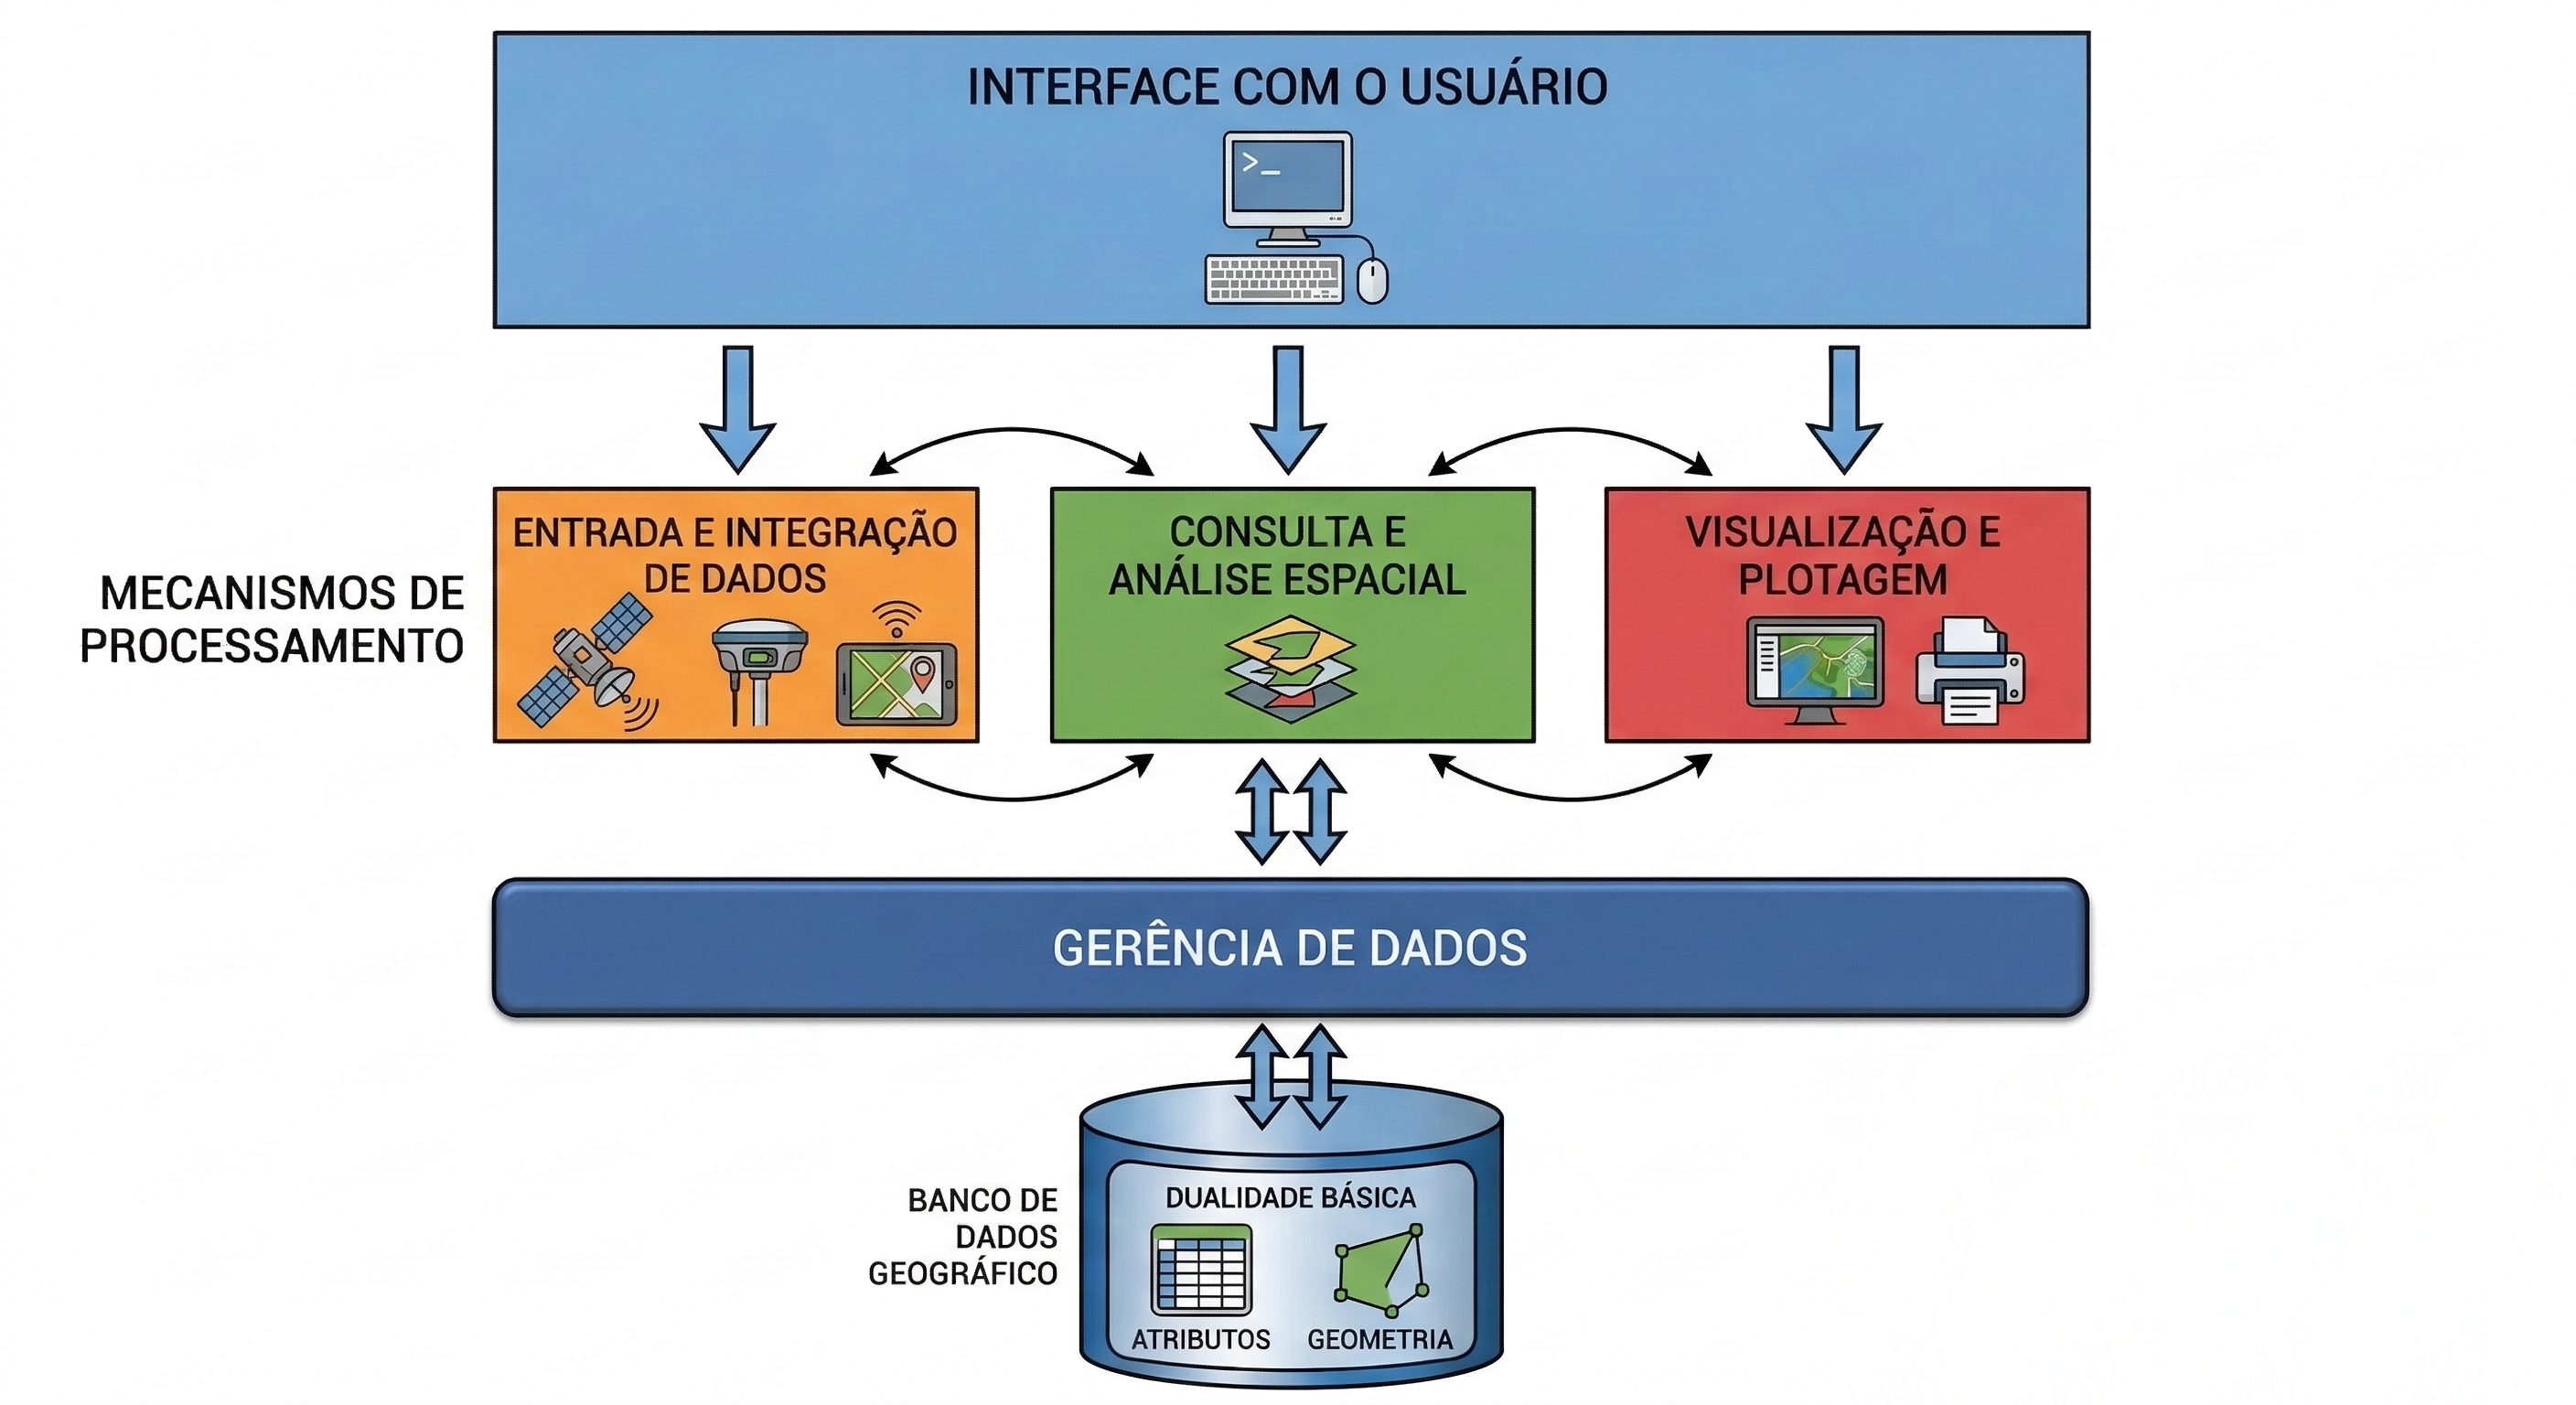
\includegraphics[keepaspectratio]{fig/arquitetura.png}}

}

\caption{Estrutura Geral de SIG. Baseado em: Câmara; Queiroz (2001)}

\end{figure}%

\bookmarksetup{startatroot}

\chapter{Dados Geoespaciais}\label{dados-geoespaciais}

In summary, this book has no content whatsoever.

\begin{Shaded}
\begin{Highlighting}[]
\DecValTok{1} \SpecialCharTok{+} \DecValTok{1}
\end{Highlighting}
\end{Shaded}

\begin{verbatim}
[1] 2
\end{verbatim}

\bookmarksetup{startatroot}

\chapter*{Referências}\label{referuxeancias}
\addcontentsline{toc}{chapter}{Referências}

\markboth{Referências}{Referências}

\phantomsection\label{refs}
\begin{CSLReferences}{0}{1}
\bibitem[\citeproctext]{ref-anselin2019}
ANSELIN, Luc. \href{https://doi.org/10.1002/9781118786352.wbieg}{Spatial
data science}. \emph{In}: RICHARDSON, Douglas (Org.). \textbf{The
International Encyclopedia of Geography: People, the Earth, Environment,
and Technology}. Hoboken, NJ: John Wiley \& Sons, 2019.

\bibitem[\citeproctext]{ref-aronoff1989}
ARONOFF, Stan. \textbf{Geographical Information Systems: A Management
Perspective}. Ottawa: WDL Publications, 1989.

\bibitem[\citeproctext]{ref-brady2007}
BRADY, Shailaja R.; SINHA, A. Krishna; GUNDERSEN, Linda C.
\textbf{Geoinformatics 2007: data to knowledge}: Scientific
Investigations Report. Reston, VA: U.S. Geological Survey, 2007.
Disponível em:
\textless{}\url{https://doi.org/10.3133/sir20075199}\textgreater.

\bibitem[\citeproctext]{ref-brodeur2001}
BRODEUR, Jean. Standardization in Geomatics: in Canada and in ISO/TC
211. \textbf{Geomatica}, v. 55, n. 1, p. 91--106, 2001.

\bibitem[\citeproctext]{ref-burrough1986}
BURROUGH, Peter A. \textbf{Principles of Geographical Information
Systems for Land Resources Assessment}. Oxford, England: Oxford
University Press, 1986.

\bibitem[\citeproctext]{ref-burrough1998}
BURROUGH, Peter A.; MCDONNELL, Rachael A. \textbf{Principles of
Geographical Information Systems}. Oxford: Oxford University Press,
1998.

\bibitem[\citeproctext]{ref-Cuxe2maraDaviMont2001}
CÂMARA, Gilberto; DAVIS, Clodoveu; MONTEIRO, Antônio Miguel Vieira.
\textbf{\href{http://urlib.net/ibi/6qtX3pFwXQZ3ukuKE/BQGus}{Introdu{ç}{ã}o
{à} ci{ê}ncia da geoinforma{ç}{ã}o}}. São José dos Campos: INPE, 2001.
p. 344

\bibitem[\citeproctext]{ref-Cuxe2maraMont2001}
CÂMARA, Gilberto; MONTEIRO, Antonio Miguel Vieira. Conceitos basicos em
ci{ê}ncia da Geoinforma{ç}{ã}o. \emph{In}: CÂMARA, Gilberto; DAVIS,
Clodoveu; MONTEIRO, Antônio Miguel Vieira (Orgs.).
\textbf{Introdu{ç}{ã}o {à} ci{ê}ncia da geoinforma{ç}{ã}o}. S{ã}o Jos{é}
dos Campos: INPE, 2001. p. 35.

\bibitem[\citeproctext]{ref-camara2001arquitetura}
CÂMARA, Gilberto; QUEIROZ, Gilberto Ribeiro de. Arquitetura de Sistemas
de Informação Geográfica. \emph{In}: CÂMARA, Gilberto; DAVIS, Clodoveu;
MONTEIRO, Antônio Miguel Vieira (Orgs.). \textbf{Introdução à Ciência da
Geoinformação}. São José dos Campos: INPE, 2001. p. 35.

\bibitem[\citeproctext]{ref-clarke2006}
CLARKE, Keith C.; PARKS, Bradley O.; CRANE, Michael P.
\textbf{Geographic Information Systems and Environmental Modeling}. 1.
ed. New Delhi: Prentice-Hall of India Pvt. Ltd., 2006.

\bibitem[\citeproctext]{ref-Gewin2004}
GEWIN, Virginia. \href{https://doi.org/10.1038/nj6972-376a}{Mapping
opportunities}. \textbf{Nature}, v. 427, n. 6972, p. 376--377, 2004.

\bibitem[\citeproctext]{ref-goodchild1992}
GOODCHILD, Michael F. Geographical information science.
\textbf{International journal of geographical information systems}, v.
6, n. 1, p. 31--45, 1992.

\bibitem[\citeproctext]{ref-hu2020}
HU, Yingjie. \textbf{Starting with data: advancing spatial data science
by building and sharing high-quality datasets}., 2020. Disponível em:
\textless{}\url{https://arxiv.org/abs/2007.08087}\textgreater{}

\bibitem[\citeproctext]{ref-Krawczyk2022}
KRAWCZYK, Artur. \href{https://doi.org/10.3390/ijgi11110557}{Proposal of
Redefinition of the Terms Geomatics and Geoinformatics on the Basis of
Terminological Postulates}. \textbf{ISPRS International Journal of
Geo-Information}, v. 11, n. 11, 2022.

\bibitem[\citeproctext]{ref-longley2015}
LONGLEY, Paul A. \emph{et al.} \textbf{Geographic Information Science
and Systems}. 4. ed. Chichester: Wiley, 2015.

\bibitem[\citeproctext]{ref-NRC2006}
NATIONAL RESEARCH COUNCIL. \href{https://doi.org/10.17226/10335}{What Is
GIScience?} \emph{In}: \textbf{Learning to Think Spatially: GIS as a
Support System in the K-12 Curriculum}. Washington, DC: National
Academies Press, 2006.

\bibitem[\citeproctext]{ref-olkedzki2004}
OLĘDZKI, Jan Romuald; KWIATKOWSKA, Joanna M. Geoinformatics-an
integrated spatial research tool. \textbf{Miscellanea Geographica.
Regional Studies on Development}, v. 11, p. 323--331, 2004.

\bibitem[\citeproctext]{ref-roberts1977}
ROBERTS, A. F.
\textbf{\href{https://books.google.com.br/books?id=Svk1AQAAIAAJ}{Geotechnology:
An Introductory Text for Students and Engineers}}. \emph{{[}S.l.{]}}:
Pergamon Press, 1977.

\bibitem[\citeproctext]{ref-Scheider2020}
SCHEIDER, Simon \emph{et al.}
\href{https://doi.org/10.1111/gec3.12537}{Why geographic data science is
not a science}. \textbf{Geography Compass}, v. 14, n. 11, p. e12537,
2020.

\bibitem[\citeproctext]{ref-tomlinson1967}
TOMLINSON, Roger F. \textbf{An Introduction to the Geo-Information
System of the Canada Land Inventory}. Ottawa, ON, Canada: Agricultural;
Rural Development Administration, 1967.

\bibitem[\citeproctext]{ref-waters2017}
WATERS, Nigel.
\href{https://doi.org/10.1002/9781118786352.wbieg0841}{GIS: History}.
\emph{In}: RICHARDSON, Douglas \emph{et al.} (Orgs.). \textbf{The
International Encyclopedia of Geography: People, the Earth, Environment
and Technology}. Chichester: Wiley, 2017.

\end{CSLReferences}




\end{document}
